\section{\textit{Android}}

	\par Segundo \citeonline{monteiro2012}, \textit{Android} é um sistema
operacional baseado em \textit{Linux} que utiliza a linguagem de programação
\textit{Java} para o desenvolvimento de seus aplicativos. Criado especialmente
para dispositivos móveis, começou a ser desenvolvido no ano de 2003 pela então
empresa Android Inc, que em 2005 foi agregada ao Google. A partir de 2007 o
projeto \textit{Android} uniu-se a \textit{Open Handset Alliance}, uma
associação de empresas de \textit{softwares}, \textit{hardwares} e
telecomunicações, que tem por finalidade desenvolver uma plataforma para
dispositivos móveis que seja completa, aberta e gratuita.

	\par \citeonline{krazit2009} afirma que o sistema pode rodar em equipamentos
de diversos fabricantes, evitando assim ficar limitado a poucos dispositivos.
Conforme informações do site \citeonline{android1}, hoje em dia existe mais de
um bilhão de aparelhos espalhados pelo mundo com esse sistema operacional.

	\par De acordo com \citeonline{monteiro2012}, as aplicações são executadas em
uma máquina virtual Java denominada \textit{Dalvik}. Cada aplicativo, usa uma
instância dessa máquina virtual tornando-o assim mais seguro. Por outro lado, os
\textit{softwares} só podem acessar os recursos do dispositivo, como uma
lista de contatos, caso seja formalmente aceito pelo usuário nos termos de uso
ao instalá-lo.

	\par As configurações de uma aplicação na plataforma \textit{Android} ficam
salvas em um arquivo XML denominado \textit{AndroidManifest.xml}, que se
localiza na pasta raiz do projeto. Para \citeonline{lecheta2010}, as informações
devem estar entre \textit{tags} correspondentes ao recurso. Para ser possível acessar a
\textit{internet} pelo aplicativo é preciso declarar a permissão de acesso da
seguinte forma: \texttt{<uses-permission
android:name="android.permission.internet" />}.

	\par \citeonline{lecheta2010} diz que as \textit{intents} são recursos tão
importantes que podem ser consideradas como o coração do \textit{Android} e que
estão presentes em todas as aplicações.	De acordo com
\citeonline[p.29]{k192012}, "são objetos responsáveis por passar informações,
como se fossem mensagens, para os principais componentes da API do
\textit{Android}, como as \textit{Activities}, \textit{Services} e
\textit{BroadCast Receivers}". \citeonline{monteiro2012} diz que as
\textit{Intents} são criadas quando se tem a intenção de realizar algo como por
exemplo compartilhar uma imagem, utilizando os APP's já existentes no
dispositivo. Existem dois tipos de Intents:
	
	\begin{itemize}
	  
	  \item \textit{Intents} implícitas: quando não é informada qual
	  \textit{Activity} deve ser chamada, ficando assim por conta do sistema
	  operacional verificar qual a melhor opção.
	  
	  \item \textit{Intents} explícitas: quando é informada qual
	  \textit{Activity} deve ser chamada. Usada normalmente para chamar
	  \textit{activities} da mesma aplicação.
	  
	\end{itemize}
	
	\par Segundo \citeonline{k192012}, uma aplicação \textit{Android} pode ser
construída com quatro tipos de componentes: \textit{Activity},
\textit{Services}, \textit{Content Providers} e \textit{Broadcast Receivers}.

	\par As \textit{activities} são as telas com interface gráfica, que permitem
interações com os usuários. De acordo com \citeonline{lacheta2013}, cada
\textit{activity} tem um ciclo de vida, uma vez que ela pode estar sendo
executada, estar em segundo plano ou totalmente destruída.

	\par Toda vez que é iniciada uma \textit{activity}, ela vai para o topo de uma
pilha denominada \textit{activity stack}. O bom entendimento de seu ciclo de
vida é importante, pois quando uma aplicação é interrompida, é possível salvar as
informações ou ao menos voltar ao estágio a qual o usuário se encontrava. Na
Figura \ref{fig:qt1} é demostrado o ciclo de vida de uma \textit{activity}.

\begin{figure}[h!]
	\centerline{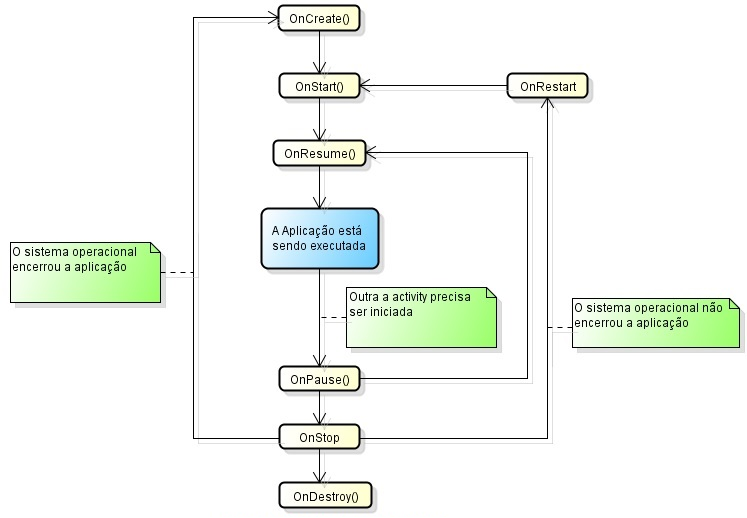
\includegraphics[scale=0.5]{./imagens/1_q_teorico/qt1.png}}
	\caption[Ciclo de Vida de uma \textit{Activity} ]{Ciclo de Vida de uma
	\textit{Activity}.
	 \textbf{Fonte:}\citeonline{lecheta2010}}
	\label{fig:qt1}
\end{figure}

	\par Para que se possa entender melhor, imagina-se o seguinte cenário: um
usuário entra no aplicativo de notas da Univás. Para que a \textit{activity}
seja criada, é chamado o método \texttt{onCreate()}, logo após é executado o
método \texttt{onStart()} e ao finalizar do ciclo anterior é chamado o
\texttt{onResume()}, só a partir de então, a \textit{activity} é visualizada
pelo discente. Contudo, durante a navegação, o aluno recebe uma ligação, então
nessa hora o sistema operacional chama o método \texttt{onPause()} para
interromper a aplicação e abrir uma outra \textit{activity} para que o usuário
possa atender a chamada telefônica. É possível, nesse método, salvar informações
que o usuário está utilizando. Ao concluir o método de pausa, é executado o
método \texttt{onStop()}, a partir de agora a \textit{activity} da Univás não
será mais visível ao usuário. Ao encerrar a ligação, há dois caminhos possíveis
de se percorrer, o primeiro, seria o caso do sistema operacional encerrar
completamente a aplicação, por necessidade de liberar espaço em memória. Dessa
forma será necessário chamar o método \texttt{onCreate()} novamente seguindo o
ciclo normal, porém se não for encerrada completamente, ao findar a ligação será
executado o método \texttt{onRestart()} e voltar para a \textit{activity} ao
qual o usuário se encontrava. Por fim ao encerrar uma \textit{activity} será
chamado o método \texttt{onDestroy()} finalizando assim o ciclo de vida.

	\par No arquivo \textit{AndroidManifest.xml}, as \textit{activities} devem
	estar entre as tags \texttt{<activity> </activity>} e a \textit{activity} principal,
ou seja, pela qual será iniciada a aplicação deve conter a tag
\texttt{<intent-filter>} além de \texttt{<action
android:name="android.intent.action.MAIN"/>} indicando que essa atividade
deverá ser chamada ao iniciar a aplicação e \texttt{<category
android:name="android.intent.category.LAUNCHER"/>}, que implica que esse
APP ficará disponível junto aos outros aplicativos no dispositivo.

	\par A \textit{Activity} a ser utilizada para iniciar a aplicação é uma
\textit{Navigation Drawer}, que segundo o site \citeonline{android2015}, que
exibe do lado esquerdo as principais funções do \textit{software}, semelhante a um
menu e fica normalmente escondida aparecendo apenas quando clicado no canto
superior esquerdo.

	\par Segundo \citeonline{lecheta2010}, a classe \textit{Service} existe
com intuito em executar processos que levarão um tempo indeterminado para serem
executados e que normalmente consomem um alto nível de memória e processamento.
Esses processos são executados em segundo plano enquanto o cliente realiza
outra tarefa. Assim um usuário pode navegar na internet enquanto é feito um
\textit{download}. O serviço é geralmente iniciado pelo \textit{Broadcast
Receiver} e quem o gerencia é o sistema operacional que só o finalizará ao
concluir a tarefa, salvo quando o espaço em memória é insuficiente.

	\par Para \citeonline{lecheta2010}, a função da classe \textit{Content
Provider} é prover conteúdos de forma pública para todas as aplicações, dessa
forma essa classe possibilita às aplicações consultar, salvar,
deletar e alterar informações no \textit{smartphone}. Assim afirma
\citeonline[p.413]{lecheta2010} “O \textit{Android} tem uma série de provedores
de conteúdo nativos, como, por exemplo, consultar contatos da agenda,
visualizar os arquivos, imagens e vídeos disponíveis no celular”. Portanto, um
contato pode ser salvo por um aplicativo e alterado por outro.

	\par Para \citeonline{lecheta2010}, a classe \textit{Broadcast Receiver}
é muito importante para a plataforma \textit{Android}, uma vez que ela é
responsável por agir em eventos de uma \textit{intent}.

	\par Essa classe sempre é executada em segundo plano, portanto, quando uma
pessoa está utilizando uma aplicação e recebe uma mensagem de SMS, o
\textit{Broadcast Receiver} capta essa informação e a processa sem a
necessidade do cliente ter que parar de realizar suas tarefas.

	\par A configuração de um \textit{Broadcast Receiver} é feita no
\textit{AndroidManifest.xml} pela \textit{tag} \texttt{<receiver>} junto com a
\textit{tag} \texttt{<intente-filter>} e conterá a rotina a ser realizada quando
for chamada. 

	\par Em uma aplicação, um elemento fundamental é a interface gráfica, que
deverá ser organizada, simples e elegante. Conforme \citeonline{monteiro2012}
esses são os principais \textit{Layouts} do sistema operacional Android:
	\begin{itemize}
	
	 \item \textit{LinearLayout}: permite posicionar os elementos em forma
	 linear, dessa forma quando o dispositivo estiver em forma vertical os itens
	 ficarão um abaixo do outro e quando estiver na horizontal eles
	 ficarão um ao lado do outro.
	
	  \item \textit{RelativeLayout}: permite posicionar elementos de forma
	  relativa, ou seja um \textit{widget} com relação a outro.
	
	  \item \textit{TableLayout}: permite criar \textit{layouts} em formato de
	  tabelas. O elemento \textit{TableRow} representa uma linha da tabela e seus
	  filhos são as células.  Dessa maneira, caso um \textit{TableRow} possua dois
	  itens, significa que essa linha tem duas colunas.
	
	  \item \textit{DatePicker}: \textit{widget} desenvolvido para a seleção de
	  datas que podem ser usadas diretamente no \textit{layout} ou através de
	  caixas de diálogo.

	  \item \textit{Spinner}: \textit{widget} que permite a seleção de itens,
	  similar ao \textit{combobox}.
	
	  \item \textit{ListViews}: permite exibir itens em uma listagem. Dessa
	  forma, em uma lista de compras, clicando em uma venda é possível listar os
	  itens dessa venda selecionada.
	
	  \item \textit{Action Bar}: um item muito importante, pois apresenta na
	  parte superior aos usuários as opções existentes no aplicativo.
	
	  \item \textit{AlertDialog}: apresenta informações aos usuários através de
	  uma caixa de diálogo. Comumente utilizado para perguntar ao cliente o que
	  deseja fazer quando ele seleciona algum elemento.
	
	  \item \textit{ProgressDialog} e \textit{ProgressBar}: utilizado quando uma
	  aplicação necessita de um recurso que levará um certo tempo para executar,
	  como por exemplo, fazer um \textit{download}, pode ser feito uma animação
	  informando ao usuário o progresso da operação.
	  
	  \item \textit{SQLite}: é um banco de dados embarcado na plataforma
	  \textit{Android}, que armazena tabelas, \textit{views}, índices,
	  \textit{triggers} em apenas um arquivo. Somente é possível acessá-lo pela
	  aplicação a qual o criou e é excluído caso o aplicativo seja removido.

	\end{itemize}
	
	\par Além dos recursos acima citados, um outro \textit{widget} que pode-se
destacar é o \textit{ExpandableListView}, que para \citeonline{android3}, exibe os
itens em forma de uma lista, similar ao \textit{ListView}, o que diferencia-o é
que ele mostra uma lista de dois níveis de rolagem vertical, em vez de abrir
uma outra tela.
	
	\par Para uma maior interação, as aplicações normalmente utilizam API’s de
terceiros, como o Google \textit{Maps}, quando necessita encontrar alguma
localização. Para \citeonline{monteiro2012} essa comunicação pode utilizar o
REST, que envia requisições através da URL. Ao receber
informações pedidas a um outro serviço, que pode estar no padrão XML ou JSON. O
REST será detalhado mais adiante.

	\par Outra ferramenta importante e muito utilizada do \textit{Android} é a
notificação. Segundo \citeonline{phillips2013}, quando uma aplicação está
sendo executada em segundo plano e necessita comunicar-se com o usuário, o
aplicativo cria uma notificação. Normalmente as notificações aparecem na barra
superior, o qual pode ser acessado arrastando para baixo a partir da parte
superior da tela. Assim que o usuário clica na notificação, ela cria uma
\textit{intent} abrindo a aplicação em questão.

	\par Com a ideia de desenvolver um aplicativo para dispositivos móveis, a
plataforma \textit{Android} foi escolhida devido ao seu destaque no mercado e
pela facilidade que apresenta aos usuários e desenvolvedores.